\documentclass[a4paper,12pt]{book}
\usepackage[utf8]{inputenc}
\usepackage{graphicx}
\usepackage{titlesec}
\usepackage{hyperref}

\titleformat
{\chapter} % command
[display] % shape
{\bfseries\Huge\itshape} % format
{\small{Tic-Tac-Toe Machine Learning Workshop}} % label
{0.5ex} % sep
{
	\rule{\textwidth}{1pt}
	\vspace{1ex}
	\centering
} % before-code
[
\vspace{-0.5ex}%
\rule{\textwidth}{0.3pt}
] % after-code





% Default fixed font does not support bold face
\DeclareFixedFont{\ttb}{T1}{txtt}{bx}{n}{12} % for bold
\DeclareFixedFont{\ttm}{T1}{txtt}{m}{n}{12}  % for normal

% Custom colors
\usepackage{color}
\definecolor{deepblue}{rgb}{0,0,0.5}
\definecolor{deepred}{rgb}{0.6,0,0}
\definecolor{deepgreen}{rgb}{0,0.5,0}

\usepackage{listings}

% Python style for highlighting
\newcommand\pythonstyle{\lstset{
		language=Python,
		basicstyle=\ttm,
		otherkeywords={self},             % Add keywords here
		keywordstyle=\ttb\color{deepblue},
		emph={MyClass,__init__},          % Custom highlighting
		emphstyle=\ttb\color{deepred},    % Custom highlighting style
		stringstyle=\color{deepgreen},
		frame=tb,                         % Any extra options here
		showstringspaces=false            % 
}}


% Python environment
\lstnewenvironment{python}[1][]
{
	\pythonstyle
	\lstset{#1}
}
{}

% Python for external files
\newcommand\pythonexternal[2][]{{
		\pythonstyle
		\lstinputlisting[#1]{#2}}}

% Python for inline
\newcommand\pythoninline[1]{{\pythonstyle\lstinline!#1!}}

\begin{document}
	
	\author{Martin Mrugała\\Patryk Walczak\\Filip Szymczak\\Bartek Żyła\\Maciej Zalewski}
	\title{\Huge{\bf{Machine Learning Workshop\\Tic-Tac-Toe Project}}}
	\date{\emph{\today}}
	
	\frontmatter
	\maketitle

	\tableofcontents
	
	\mainmatter
	\chapter{Introduction}
	\section{Standard Tic-tac-toe}
	According to the definition in the Oxford Dictionary of English, Tic-tac-toe is a game in which two players seek to complete a row of either three noughts or three crosses drawn alternately in the spaces of a grid of nine squares.
		\begin{figure}[!h]
		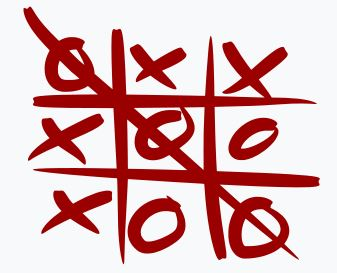
\includegraphics{./Images/1.jpg}
		\centering
		\caption{A completed game of Tic-tac-toe\protect\footnotemark.}
		\label{fig:Capture1}
	\end{figure}
	\footnotetext{Source of the image: \url{https://en.wikipedia.org/wiki/Tic-tac-toe}}
	And as it turns out, there are 255 168 possible games. So this means that, with the help of the reinforcement learning, a bot may train to mastery. 
	\newpage
	\section{Our implementation}
	Our team decided to create a bot which would play this game but in an expanded version of it. The principal changes concern, inter alia:\\
	\begin{itemize}
		\item \textbf{The size of the grid could be infinite}\\
		The number of squares is not boundless, of course. Due to the CPU, as well as the storage limitations, the infinity has to be simulated. We came up with two solutions. The first one is pretty straightforward, but a little preachy. The idea is to set the size in advance. The second one, in turn, assumes an increase in the size whenever the players get close to the edge.
		\item \textbf{Condition of winning}\\
		The length of the sequence of X's or O's needed to win may have any value. Naturally, it has to satisfy the following condition:
		\begin{center}
			$0 < length < edgelength$
		\end{center}
		There is still the matter of the draw. In case of the constant size gird, the tie occurs, whenever there is no way for any player to win.
	\end{itemize}
	\section{Machine Learning backgroud}
To deal with the problem we are using reinforcement learning, which trains algorithm by a system of reward and punishment. In this way we can put one bot against the other and let them play, so they will find the best solutions by themselves without any supervision. 
\\Basic reinforcement learning can be modeled as a Markov decision process:
	\begin{itemize}
		\item set of states $S$ (state space)
		\item set of actions $A$ (action space)
		\item reward $R$ after transition from state $s$ to $s'$ under action $a$
		\item probability of transition from state $s$ to $s'$ under action $a$
	\end{itemize}
\pagebreak

\begin{figure}[!h]
	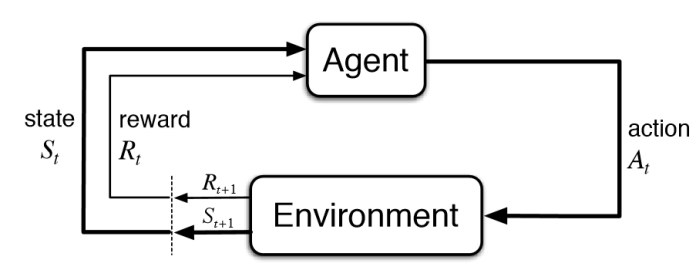
\includegraphics{./Images/RLdiag.jpg}
	\centering
	\caption{Decision process diagram\protect\footnotemark.}
	\label{fig:Capture1}
\end{figure}
\footnotetext{Source of the image: \url{https://www.kdnuggets.com/images/reinforcement-learning-fig1-700.jpg}}

A reward is a scalar feedback signal, which indicates how well agent is doing at the given step $R_{t}$. Reinforcement is based on the reward hypothesis, which tells that goals can be described by the maximisation of expected cumulative reward, so the agent's job is to maximise cumulative reward. To do so, in our implementation, it selects actions, which gives the greatest reward (have the greatest value) immediately. 
\\Observation is the information about environment received by the agent. The history is the sequence of observations, actions and rewards up to time $t$.

\begin{equation}
	H_{t} = A_{1}, O_{1}, R_{1}, ...,  A_{t}, O_{t}, R_{t}
\end{equation}

State is the information used to determine the next action. Our environment (game board) is fully observable, so the state of environment is the same as the state of the agent and observation of the agent. State can be described as a function oh history.

\begin{equation}
	S_{t} = f(H_{t})
\end{equation}

A state $S_{t}$ is Markov state if and only if

\begin{equation}
	P[S_{t+1} | S_{t}] = P[S_{t+1} | S_{1}, ..., S_{t}]
\end{equation}

Then if the current state is known, the history is not needed. State $S_{t}$ is enough to decide on the next action.
\\




	\chapter{Solution}
	\section{Algorithms and data processing functions}
Bot algorithm is trained against the other instance of the bot at the beginning, then the winner is chosen by comparing the number of wins and forwarded to the player as the best current solution. Iterations are the number of games to play between bots - the more they play, the better they are.
	
\begin{python}
def train(iterations):
	player1Win = 0.0
	player2Win = 0.0
	loadPolicy()
	for i in range(0, iterations):
		play()
		if (player1 wins):
			player1Win += 1
			player1.feedReward(1)
			player2.feedReward(0)
		if (player2 wins):
			player2Win += 1
			player1.feedReward(0)
			player2.feedReward(1)
		if (draw):
			player1Win += 1
			player1.feedReward(0.1)
			player2.feedReward(0.1)
	savePolicy()
	if (player1Win > player2Win):
		return player1
	else:
		return player2
\end{python}

Limiter in the bot instance limits the range of the optional moves on the board. ExploreRate is a probability of a random action, stepSize controlls increasement of the value for the given state during reward feeding. 
\\In this function, the set of actions is constructed for a given state. AI decides which move to make by considering every possibility in it's current bounds. The move is analyzed by checking how the state would look like after the action. If such situation on the board has not occured before (it is not in the estimations), the new state is given the value (1 for win, 0 for lose and 0.5 otherwise), hashed and added to the estimations dictionary.

\begin{python}
def move(state):
    nextStates[ ]
    nextPositions[ ]
      for i in range (-limiter, limiter+1):
        for j in range (-limiter, limiter+1):
          if move is possible:
            nextPositions.append((i,j))
            nextStates.append(nextState(i,j).getHash())
            if nextState(i,j).getHash() not in estimations:
            if nextState(i,j).isEnd:
              if win:
                estimations[nextState(i,j).getHash()] = 1
              else:
                estimations[nextState(i,j).getHash()] = 0
            else:
              estimations[nextState(i,j).getHash()] = 0.5
\end{python}
 
After calculations the decision has to be made. There is a chance to perform a random action (probability of this is given by exploreRate), which allows to explore new paths with a possibility of finding a new, better tactic. Otherwise the action with the biggest value based on the previous training is chosen.

\begin{python}
if random.binomial(1, exploreRate):
	r = random.(0, length(nextPositions)-1)
	action = nextPositions[r]
	states.append(nextStates[r])
	return action

values = [ ]
for hash, position in (nextStates, nextPositions):
	values.append((estimations[hash], position))
v = value.index(max(values.estimation))
action = values[v][1]
states.append(nextStates[v])
return action	
\end{python}

Upon finishing the game iteration, algorithm is fed with the reward according to the result. Values for states from the path chosen in the current iteration are adjusted starting from the last one. The change depends on the "size" of the reward, stepSize and values of previously rewarded states along the path when going back. \\That is how the algorithm learns which paths are better to choose and which ones should be rather ommited. If the outcome was positive, values will be slightly increased. If the game was lost, values will drop down a little bit. The changes are scaled so they are small and do not affect strongly the possibility of choosing other paths. Parameters can be changed to find the optimal way of learning.

\begin{python}
def feedReward(reward):
  if length(states) == 0:
    return
  target = reward
  for latestState in reversed(states):
    value = estimations[latestState] 
		+ stepSize * (target - estimations[latestState])
    estimations[latestState] = value
    target = value
\end{python}

There are two policies, optimal policy 1 is for the starting bot and optimal policy 2 is for the bot which has second move. Each training session starts with loading the last optimal policy as estimations and ends with saving them. 
	\\The file contains hashed states, which allows for a quick comparison as keys, and their appropriate values in a dictionary. In this way we do not have to store and compare the whole state, calculating hash is enough to preserve the uniqueness of the state. Only the list of moves, in proper order for the given state, is being hashed. Stored data should be reduced to the necessary minimum because the number of possible states grow very quickly (for the infinite board there are infinite states).

\begin{figure}[!h]
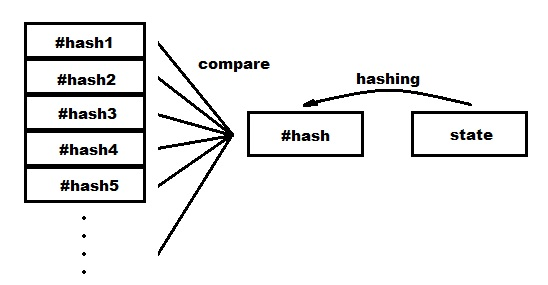
\includegraphics{./Images/hashing.jpg}
	\centering
	\caption{Comparision of a given state with the estimations.}
	\label{fig:Capture1}
\end{figure}



	\chapter{Code}
	\begin{python}
		class MyClass(Yourclass):
		def __init__(self, my, yours):
		bla = '5 1 2 3 4'
		print bla
	\end{python}
	\chapter{Bibliography}

	
	\backmatter
	% bibliography, glossary and index would go here.
	
\end{document}